\documentclass[a4paper,12pt]{article}
\usepackage[latin1]{inputenc}     % pour Unix Latin1 aussi..
% \usepackage[applemac]{inputenc} % pour utilisateurs mac
% \usepackage[ansinew]{inputenc}  % pour Windows ANSI (yen a encore qui utilisent ca? :s)
\usepackage{verbatim} 
\usepackage{aeguill}
\usepackage{amsfonts}
\usepackage{xspace}
\usepackage{amsmath}
\usepackage{lscape} % pour avoir une page en paysage
\usepackage{fancybox}
\usepackage{fancyhdr}
\usepackage{textcomp}  % pour les caract�res sp�ciaux (copyleft etc)
\usepackage{marvosym} % caractere electrostatic, laserbeam...
\usepackage{supertabular}% tableaux sur plusieurs pages
\usepackage{ifsym} % caract�res scp�ciaux
\usepackage{longtable}
\usepackage{upgreek}
\usepackage{picins}
\usepackage{lastpage}
\usepackage[english,french]{babel}
%%%%%%%%%%%%% parallel, multicolpar et parcolumns.%%%%%%%%%%%%%%%%%%%%%% pour des documents multicolones bilingue.
\usepackage[pdftex]{graphicx, color}
\usepackage{pdfpages}
\graphicspath{{img/}} % La ou j'ai mes images
\DeclareGraphicsExtensions{.jpg,.png}
\pdfoutput=1
\usepackage[pdftex,
	a4paper,
        bookmarks = true,           % Signets
        bookmarksnumbered = true,   % Signets numerotes
        pdfpagemode = None,         % Signets/vignettes fermes a l'ouverture
        %pdfstartview = FitH,        % La page prend toute la largeur
	pdfstartview = FitV,        % La page prend toute la hauteur
	colorlinks=true,
	citecolor=black,urlcolor=blue,linkcolor=red,
	pdfauthor={K�vin Raymond},
	pdftitle={Stage au CERN},
 	pdfsubject={Rapport de stage},
	pdfkeywords={Xbee, pt100, PIC, GNU,Piklab, SDCC, Linux, CAO, gEDA},
	plainpages=false,
	pdfpagelabels,
	bookmarks,
	breaklinks=true,
   	hyperindex,
	linktocpage=true	% pour colorier seulement le num�ros dans la TOC	
]{hyperref}
%
\pdfcompresslevel=9
%
%
%%% style sans serif pour les url
\urlstyle{sf}

%



%%%% debut macro %%%%
\newenvironment{changemargin}[2]{\begin{list}{}{%
\setlength{\topsep}{0pt}%
\setlength{\leftmargin}{0pt}%
\setlength{\rightmargin}{0pt}%
\setlength{\listparindent}{\parindent}%
\setlength{\itemindent}{\parindent}%
\setlength{\parsep}{0pt plus 1pt}%
\addtolength{\leftmargin}{#1}%
\addtolength{\rightmargin}{#2}%
}\item }{\end{list}}
%%%% fin macro %%%%

%
%
%%%%%%%%% Mise en Forme page de garde %%%%%%%%%%%%%%%%%%%%
%######################## D�finition du titre ######################
\title{
\thispagestyle{empty}
\vspace{-40mm}
   \begin{minipage}[c][150pt][c]{.40\linewidth} %[hauteur][position]{largeur}
		\begin{flushleft}
		\vspace{2mm}
		\includegraphics[width=3cm]{./img/CERN_logo}
		\vspace{3mm}
		\end{flushleft}
   \end{minipage}\hfill
   \begin{minipage}[c][150pt][c]{.40\linewidth} %[hauteur][position]{largeur}
	{\normalsize 
		\begin{flushright}
		\vspace{3mm}
		\textsc{K�vin Raymond}\\
		Ann�e 2007\\
		\end{flushright}
	}
   \end{minipage}
\vfill
\rule{\linewidth}{0.8mm}\vspace{6mm}\\
    \begin{minipage}[c]{0.70\linewidth} %[hauteur][position]{largeur}
	{\large	
		Utilisation de gEDA, suite libre de CAO\\
		Programmation des PIC sous Linux\\
		Utilisation de la carte Mesure de temp�rature\\
	}
	\end{minipage}\vspace{6mm}
\rule{\linewidth}{0.8mm}\vspace{6mm}\\
\vspace{3mm}
\begin{minipage}[c][150pt][c]{.40\linewidth} %[hauteur][position]{largeur}
	{\normalsize 
		\begin{flushleft}
		\textbf{R�sum�~:}\\
		Article d�stin� � aider � prendre en main la suite de CAO gEDA, Piklab pour programmer les PIC sous linux et quelques notes sur l'utilisation de la carte pour mesurer les temp�ratures.
		\end{flushleft}
	}
   \end{minipage}
\date{} % Je ne veux pas afficher la date
}  %fin du titre



%
%%%%%%%%%%%%%%%% Fin des includes... %%%%%%%%%%%%%

\begin{document}

%%
\maketitle

\newpage

\setcounter{page}{1} %On definit un compteur a 1
\pagenumbering{roman} %permet une num�rotation en chiffre romain

%%
\tableofcontents
\newpage



\setcounter{page}{1} % On r�initialise le coompteur des pages
\pagenumbering{arabic} % On repasse en num�rotation en chiffre Arabe
\pagestyle{fancy}
\chapter*{Introduction}
\addcontentsline{toc}{chapter}{Introduction}
\section*{G�n�ralit�s}
Etudiant en deuxi�me ann�e � l'Institut Universitaire et Technologique (IUT) d'Annecy en G�nie Electrique et Informatique Industrielle (GEII), j'ai �t� amen� � r�aliser un stage d'une dizaine de semaines pour d�couvrir le monde industriel et un domaine d'activit�s. Je l'ai effectu� au sein du CERN du 2 avril au 22 juin 2007. 
Ce stage a �t� une opportunit� pour moi de travailler dans un centre de recherche. Le but �tant non pas le profit mais l'avanc�e scientifique, cela cr�e une r�elle motivation.

C'est dans ce cadre que j'ai mis en pratique mes connaissances acquises ces derni�res ann�es, mais �galement appris � m'adapter pour optimiser et non plus appliquer pour r�aliser. 



\section*{Cahier des charges}
Ne s'agissant pas d'une t�che critique, j'avais pour but de r�aliser un projet pouvant facilement �tre repris pour mieux l'adapter aux besoins du CERN. \newline

Il consiste en deux cartes~: l'une mesurant la temp�rature avec le plus de pr�cision possible (0,1 \degres C), la seconde recevant les temp�ratures pour les enregistrer sur un ordinateur qui devra les traiter.
La carte de mesure de temp�rature devant �tre aliment�e par une pile (9V), sa consommation doit �tre minimale.
Ces deux cartes doivent �tre en liaison sans fil avec une port�e raisonnable.

Le choix du capteur est libre, tout en respectant la pr�cision sur une plage mesure de 0~\degres C � +30~\degres C.
Le protocole utilis� pour la transmission sans fil est libre mais doit �tre fiable et d'une faible consommation.
Pour ce qui est de la r�ception sur l'ordinateur, le protocole est �galement libre.

Il doit �galement �tre possible d'avoir plusieurs satellites (carte de mesure pour la temp�rature) � divers endroits �mettant les informations vers l'ordinateur.

Une contrainte plus restrictive est d'explorer le monde du logiciel libre. Pour ce qui est de la r�alisation de la carte et du d�veloppement logiciel, j'ai explor� ce domaine sur une machine GNU/Linux.

Cela m'a �galement permis de me familiariser avec Linux.\newline


    Apr�s avoir pr�sent� le CERN, nous nous int�resserons � mon activit� de stagiaire ainsi qu'aux travaux r�alis�s, et enfin nous
ferons le bilan de ce stage avant de conclure sur sa globalit�. 


 \newpage
\section{gEDA}
Les logiciels de Conception �lectronique Assist� par Ordinateur (CAO) propri�taires sont une bonne solution pour d�buter rapidement et obtenir simplement des cartes exploitables. 

Mais ne serait-il pas plus souhaitable d'utiliser un outil compl�tement personnalisable avec lequel on n'obtient tr�s rapidement des cartes au rendu professionel~? Ceci est possible gr�ce aux logiciels libres. gEDA en est id�al pour la CAO. C'est un outil en plein d�veloppement mais d'ores et d�j� �volu�. 

De nombreuses librairies sont disponibles et il est tr�s rapide d'en ajouter. Il en existe deux m�canismes. Le premier appel� \og Oldlib \fg\, \og pcblib \fg\ ou \og biblioth�que M4 \fg\ d�pend du langage macro M4. Les empreintes sont g�n�r�es � la vol�e. \` A utiliser pour creer rapidement des familles d'empreintes. Le deuxi�me m�canisme est appel� \og Newlib \fg . Ce sont les empreintes que l'on peut creer graphiquement avec Pcb, ou avec un �diteur de texte (code ASCII). \newline

gEDA pour GPL Electronic Design Automation est une suite Open Source permettant la cr�ation de sch�mas, la simulation et la r�alisation du Printed Circuit Board (PCB). \newline

Cette suite d'outils est principalement compos�e de :
\begin{itemize}
\item[-] \textbf{gschem}, l'�diteur de sch�mas et de symboles,
\item[-] \textbf{gnetlist}, un translateur vers d'autres utilitaires,
\item[-] \textbf{PCB}, un outil de dessins de circuits imprim�s et de cr�ation d'empreintes,
\item[-] \textbf{ngspice}, un clone de spice avec des fonctions �tendues,
\item[-] \textbf{gnucap}, un simulateur original avec compilateur de mod�les,
\item[-] \textbf{geda}, le gestionnaire de projet (non actuel).
\end{itemize}

\vspace{5mm}
Attention � l'utilisation de geda le gestionnaire de projet. Il n'a pas suivi l'�volution des autres programmes, il est donc pr�f�rable de ne pas l'utiliser. Un terminal suffit pour relier les diff�rents outils.\newline

%%

\subsection{installation}
Avant tout il faut l'installer. La derni�re version de gEDA n�cessite python 2.5 ou sup�rieur. Il est possible que gEDA, ainsi que toutes ses d�pendances, soit dans les d�p�ts de votre distribution (voir par exemple avec Synaptic). Mais ce ne sera peut-�tre pas la derni�re version. Pour cette suite en constante �volution il est important d'avoir la derni�re version, pour �viter certains bogues.\newline


Une autre possibilit� est de t�l�charger l'image iso du CD. Elle inclut la derni�re version de tous les programmes. Ainsi que les d�pendances n�cessaires. Voir dans la partie download du site officiel : \url{http://www.geda.seul.org/}\label{sitegEDA}. La solution la plus simple est de monter le cd sur un lecteur virtuel. Tr�s simple sous linux.
\begin{center}
\ovalbox{\$ sudo mount -oloop <image>.iso /mnt} 
\end{center}
\vspace{2mm}

Pour poursuivre l'installation l'aide n�cessaire se trouve sur le CD. En ce qui concerne les tutoriaux, attention � bien lire les derni�res versions.\newline


Une fois l'installation termin�e, il faut avoir le synoptique de la suite logicielle en t�te pour commencer une carte.
\begin{center}
\begin{figure}[h!]
	\includegraphics[width=8cm]{./img/gedaSy}
	\caption{Synoptique de la suite gEDA}
\end{figure}
\end{center}
\vspace{2mm} 

Tout commence avec gschem. Une fois le sch�ma r�alis� et v�rifier avec le contr�leur DRC il faut cr�er la netliste. Grenum sert � assigner une r�f�rence � tous les composants. Ce qui peut �tre r�alis� automatiquement avec gschem. De m�me gattrib permet d'assigner des empreintes aux composants. Mais il est plus �vident au d�but de le faire sous gschem. 
gsch2pcb permet de cr�er la netlist et le fichier *.pcb. Pcb permet de placer les composants et de router les connexions g�n�r�es par la netlist. Enfin, les fichiers Gerber sont export�s par Pcb.


%%
\subsection{gschem}
gschem est un logiciel permettant de rapidement cr�er des sch�mas pour peu que nous l'ayons bien en main. Il existe une multitude de raccourcis permettant d'aller plus vite. \newline

Il est conseill� de cr�er un dossier de projet, car de nombreux fichiers seront cr��s. Une fois gschem ouvert (commande \og gschem\fg), vous verrez une interface simple d'utilisation~: seulement quelques ic�nes sont dans la barre des t�ches. Possibilit� d'ajouter des composants, de cr�er des fils de connexion voire des bus de donn�es. Pour tourner les composants ou toute autre t�che utile, il est bien plus rapide de se servir des raccourcis.
gschem �tant en fran�ais, il est tr�s rapide de trouver les fonctions d�sir�es.\newline

En vue de simplifier la g�n�ration de la netlist, veuillez � bien renseigner au minimum trois champs importants pour gschem. 

Double-cliquer sur un composant pour ouvrir ses propri�t�s. En g�n�ral le champ \textbf{device} et  \textbf{refdes} est rempli. Le champ de loin le plus important est \textbf{footprint}, il permet de sp�cifier quelle empreinte prendre pour ce composant. N'importe quel symbole (ou composant) peut appeler n'importe quelle empreinte. Cela permet de cr�er une seule empreinte pour plusieurs composants. Ils seront diff�renci�s sous Pcb par leur identifiant device et refdes. Une fois les composants ajout�s, il est possible de renseigner automatiquement tous les champs refdes par \og Attributs -> Annotation automatique\fg. Les champs slot et numslot permettent de sp�cifier le num�ro de la porte  lorsqu'il y en a plusieurs par bo�tier.\newline

Lors de la cr�ation de symboles il faut sp�cifier le champ \textbf{pintype} pour que le v�rificateur d'erreurs (DRC) puisse v�rifier les erreurs de connexions. Les diff�rentes options pour ce champ sont \og io\fg\ pour une entr�e-sortie, \og pas\fg\ pour une broche passive, \og in\fg\ pour une entr�e, \og out\fg\ pour une sortie et \og pwr\fg\ pour une alimentation.\newline

Une fois que le sch�ma est fini, il faut le v�rifier avec le DRC puis corriger les erreurs. Lancer le code ci-dessous dans un terminal au m�me endroit que votre projet.

\begin{center}
\ovalbox{\$ gnetlist -g drc2 text.sch -o drc\_output.txt} 
\end{center}

le r�sultat de DRC est visible dans le fichier drc\_output.txt. \newline

Personnellement, je trouve plus simple de lire le r�sultat directement dans la console:
\begin{center}
\ovalbox{\$ gnetlist -g drc2 text -o -} 
\end{center}

Si vous rencontrez une erreur du type 

\begin{quote}
Checking slots~\dots\newline
ERROR: Reference U5: Slot out of range (1).\newline
slotnumber~=~1\newline
\end{quote}

Vous avez s�rement une empreinte avec un nom finissant par une minuscule. Ce qui est interpr�t� comme le num�ro d'une porte logique � l'int�rieur d'un composant. S'il ne s'agit pas d'une erreur il est possible de passer outre en sp�cifiant le champ \textbf{numslot} � 0.\newline


La netlist est cr�e en m�me temps que le rapport du DRC, il faut donc maintenant invoquer gsch2pcb pour commencer le routage.
\begin{center}
\ovalbox{\$ gsch2pcb -v text.sch} 
\end{center}
L'option verbose (-v) est facultative, mais permet de suivre les diff�rentes erreurs dues principalement � des empreintes introuvables. La double option verbose (\$~gsch2pcb~-v~-v~text.sch) permet de voir tous les fichiers scann�s pour trouver les diff�rentes empreintes.
Lorsqu'il n'y a plus d'erreurs, il faut passer sur Pcb. Le fichier text.pcb est cr�� par gsch2pcb. Il faut maintenant l'ouvrir avec Pcb.\newline

Je pr�cise que les principales d�marches � suivre sont rappel�es par gsch2pcb � la fin du rapport. Lors d'une premi�re ex�cution on peut lire par exemple:

\begin{quote}
Next step:
\begin{itemize}
\item[1.]  Run pcb on your file test.pcb.
    You will find all your footprints in a bundle ready for you to place
    or disperse with \og Select -> Disperse all elements\fg\ in PCB.

\item[2.] From within PCB, select \og File -> Load netlist file\fg\ and select 
    test.net to load the netlist.

\item[3.] From within PCB, enter
		:ExecuteFile(test.cmd)\newline
\end{itemize}
\end{quote}
 

Lors d'une mise � jour (le fichier test.pcb existe d�j�) d'autres conseils apparaissent :
\begin{quote}
Next steps:
\begin{itemize}
\item[1.] Run pcb on your file test.pcb.
\item[2.] From within PCB, select \og File -> Load layout data to paste buffer\fg\
    and select test.new.pcb to load the new footprints into your existing layout.
\item[3.] From within PCB, select \og File -> Load netlist file\fg\ and select 
    test.net to load the updated netlist.

\item[4.]From within PCB, enter
           :ExecuteFile(test.cmd)\newline
\end{itemize}
\end{quote}


Dans tous les cas la prochaine �tape est Pcb.


%%%%
\subsection{Pcb}
\parpic[r]{\includegraphics[width=25mm]{./img/pcb}}Je conseille d'ouvrir directement Pcb par un autre terminal puisque le programme retourne un certain nombre d'erreurs (notamment \og unknown action\fg\ pour une commande inconnue) . Proc�der par \ovalbox{\$~pcb~test.pcb} tout en �tant dans le r�pertoire du projet.\newline
Pcb ouvre automatiquement une fen�tre de log qui retourne les diff�rentes actions de l'utilisateur prises en compte par le programme.\newline

Une fois le fichier test.pcb ouvert il faut r�organiser les composants (Select -> Disperse all elements).
Il ne reste plus qu'� importer la netlist (File~->~Load netlist file). Ensuite lancer le fichier test.cmd par l'invite de commande (le raccourci pour cette action est [:]). \ovalbox{ExecuteFile(test.cmd)}. Puis remettre � jour. Action possible par la touche de raccourci [O]. 
Si les fils de connexions (ratsnet) ne sont pas visibles, activer l'option en cliquant sur le bouton \og ratsnet\fg\ (� gauche).\newline

\begin{center}
\shadowbox{
\begin{minipage}{0.7\textwidth}
Pour mettre � jour le PCB si un changement doit appara�tre (modification sous gschem des connexions ou composants par exemple), lancer le DRC pour v�rifier et r�g�n�rer la netlist, ce qui a pour effet de cr�er un fichier test.pcb.new. Ouvrir ce fichier par \og File -> Load layout-data to past buffer \fg. Recharger la netlist, lancer la commande ExecuteFile(test.cmd) et r�actualiser les fils de connexions ([O]). 
\end{minipage}
} \newline
\end{center}



{\Large Pour une prise en main assez rapide de Pcb:\newline}

Dans la barre d'outils verticale (sur la gauche) il est possible de s�lectionner l'affichage des plans, via, pistes etc. Par d�faut il existe plusieurs couches avec une couleur pour chaque signal (alimentation, donn�es~\dots). Il est possible de modifier ces options par \og File -> Preference\fg.

En dessous sont repr�sent�s les outils de dessins. Line pour les pistes, polygon pour les plans de masses par exemples, LOCK pour v�rouiller un composant. Utile par exemple pour les plans ou les gros composants, cela �vite de le s�lectionner alors que l'ont visait une piste. L'outil THRM permet rapidement d'ajouter ou d'enlever des freins thermiques aux pastilles.

Pour d�placer un composant avec ses pistes (ou ratsnet), le clic souris suffit. Parfois il est pr�f�rable de d�placer un composant sans ses connexions. Pour cela il faut le s�lectionner (clic souris) puis le d�placer par un autre clic souris.

Plusieurs actions sont disponibles par [shift]+Clic droit. Notamment supprimer l'ensemble de la s�lection.
La touche [Shift] lors d'un trac� de piste sert � modifier la position de l'angle. Tr�s pratique!

Pour une mesure rapide [CTRL]+[M] r�-affecte l'origine (les mesures sont en haut � droite). Pour avoir la vue de la face de dessous il suffit de presser la touche [TAB]. Alors que [B] permet de passer le composant d'une face � l'autre. 

[U] pour \og Undo\fg\ (annuler) et [Shift]+[R] pour \og Redo\fg\ (restaurer). 

[Q] permet de modifier l'apparence des pastilles (rondes ou carr�es).[D] permet d'afficher rapidement le num�ro des broches et [shift]+[D] en donne l'apper�u. 

[O] qui permet de r�actualiser les connexions est souvent utilis�e de m�me que [F] qui permet de mettre en surbrillance les connexions directes. [S] et [shift]+[S] servent � modifier la taille des pastilles, pistes, etc. 

[V] permet d'avoir une vue globale de la carte. Pour le reste des raccourcis utilis�s, voir dans \og Window -> Key References\fg.\newline

Attention � bien activer l'option \og Settings -> New lines, arcs clear polygon\fg\ si vous devez faire un plan de masse ou autre par la suite. \` A d�faut vous retrouverez toutes vos pistes court-circuit�es par le plan. Attention cela pose probl�me pour les freins thermiques. Citation: \og � consommer avec mod�ration\fg.

Cependant il est toujours possible d'activer l'option � la fin,  un travail assez r�barbatif.
Dans les tutoriaux on peut trouver la commande \og :changejoin(selected)\fg\ pour changer l'option sur toutes les pistes s�lectionn�es, mais cela n'avait aucun effet sur ma version. D�couvert par le \og unknown action\fg\ retourn� dans le terminal. La touche raccourci pour le m�me r�sultat est [shift]+[J]. Il est possible de modifier la clearance des pistes (espace vide entre la piste et le plan) par la touche [K] (et [shift]+[K]).\newline

Lorsque vous avez le programme en main, il est tr�s rapide de router ses cartes puisque le logiciel permet d'un clic de copier des �l�ments dans un tampon (�l�ments pr�c�demment cr��s). On peut donc avoir � port�e de clic des dessins souvent utiles (logo, empreinte de frein thermique, etc.)\newline

{\Large Cr�er des empreintes (Footprint):}\newline 

Partir d'un �l�ment existant est le plus rapide. Il est possible (et tr�s utile, pour v�rification notamment) de cr�er des empreintes directement sur notre PCB. 

Pour ce faire, ouvrir le gestionnaire de librairie par \og Window~->~library\fg. Ajouter le composant le plus ressemblant. Le s�lectionner pour ensuite le copier dans le buffer ([CTRL]+[X]). Maintenant il faut le convertir en \og pi�ce\fg\ : \og Buffer~->~Convert~buffer~to~pieces\fg. Coller cette pi�ce. 

Il est maintenant possible de jouer avec tous ces �lements. Num�roter les broches avec la touche [N]. Une fois toutes les modifications effectu�es, copier la pi�ce dans le buffer puis \og Buffer~->~Convert~buffer~to~elements\fg\ pour enfin l'enregistrer \og Buffer~->~Save~buffer~to~File\fg.

Noter que les pastilles \og carr�es\fg\ sont obtenues par des lignes \og arrondies\fg\ et ensuite modifi�s avec la touche [Q] (une fois converties en �lement).\newline

\textbf{Attention, si le nom des empreintes contient une minuscule comme dernier caract�re, elle sera consid�r�e comme une porte � l'int�rieure d'un autre composant (souvent nomm�e a, b, c~\dots) Elles seront ignor�es. Il faut mettre un chiffre ou une majuscule.}\newline

Pour plus d'informations : \newline
\url{http://ronja.twibright.com/guidelines/footprints.php}, pour une plus grande explication sur la cr�ation d'empreintes graphiques (par Pcb).\newline
\url{http://www.brorson.com/gEDA/land_patterns_20050129.pdf}, un tutoriel pour dessiner ses empreintes � la main, avec un �diteur de texte.\newline




Une fois le PCB termin�, d'un clic on peut exporter la carte en fichier Gerber, png, ps, eps~\dots 



%\section{Conclusion sur gEDA}

Une des plus grandes richesses de gEDA est le traitement des donn�es entre les diff�rents programmes. Tous les fichiers sont en ASCII ce qui les rend tr�s facile � manipuler. Il est donc possible de se cr�er des scripts pour automatiser des t�ches r�barbatives. Habituellement le Perl est utilis� pour cela. Voici les scripts distribu�s par gEDA~:\newline
\begin{itemize}
\item[1.] John Luciani poss�de un large �ventail de scripts disponibles sur son site we (\url{http://www.luciani.org/}). Dans cette collection, des scripts sont inclus pour g�n�rer des empreintes, notamment Footgen.
\item[2.] David Rowe poss�de des scripts pour mettre � jour des �l�ments de m�me qu'ajouter/supprimer des fichiers PCB les uns des autres sur son site web (\url{http://www.rowetel.com/perl4pcb.html}).
\item[3.] Stuart Brorson a �crit un script simple qui g�n�re des empreintes pour deux ponts thermiques passifs en SMD. Un tarball gzipp� est disponible � \url{http://www.brorson.com/gEDA/Smtgen.pl.gz}.\newline
\end{itemize}


Une fois en main, gEDA est � la fois simple et rapide � utiliser. De plus beaucoup de librairies sont disponibles sur \textbf{\url{http://www.gedasymbols.org/}}. Il est �galement possible de demander sur la liste des geda-user si ce composant est disponible. Pour cela voir \url{http://geda.seul.org/mailinglist/index.html}. \newline

Pour la recherche de librairies, suivre les liens pr�c�demment cit�s ou \textbf{\url{http://www.gedasymbols.org/}}. On en apprend �galement beaucoup sur \url{http://www.geda.seul.org/wiki/geda:usage.fr}.\newline

Sur divers sites internet on trouve des tutoriaux pour gEDA, mais en g�n�ral ils ne sont pas � jour. Tout le probl�me est l�. Les plus int�ressants sont les tutoriaux des logiciels et non de la suite. Eux sont � jour. Je pense par exemple au tutorial de Pcb disponible sur \url{http://pcb.sourceforge.net/manual.html}. Pour comprendre un peu mieux la gestion d'un projet sous gEDA il peut �tre utile de lire le tutorial en Fran�ais disponible l�~: \url{http://www.iznogood-factory.org/pub/gEDA/tutorialfr.html}. Il n'est pas bas� sur la derni�re version, car certaines configurations ont chang�es. Sur ce site (\url{http://ofset.sourceforge.net/freeduc/book/book_29.html}) est disponible un exemple rapide de prise en main de Pcb. En lisant plusieurs tutoriaux dont la version n'est plus � jour, il est plus simple de voir ce qui est toujours d'actualit�. Pour une aide � la cr�ation d'empreinte, voir~: \url{http://www.iznogood-factory.org/pub/gEDA/land_patterns_fr.pdf}.\newline

Ce qui peut perturber au d�but c'est la profusion de raccourcis. Tant pour gschem que pour Pcb. Attention � ne pas tester toutes les touches sans v�rifier au risque de voir plus tard que la grille a �t� modifi�e, que le pas n'est plus en inch mais en millim�tres, etc. A noter �galement que les racourcis sont diff�rents suivant les programmes. 

Le seul inconv�nient notable de gschem est la fonction \og undo\fg. Lorsque l'on annule les derni�res op�rations, le zoom est pris en compte.\newline

gEDA est donc une suite tr�s compl�te. Sa principale difficult� de prise en main repose sur le fait que les tutoriaux ne sont pas � jour. Il faut pr�f�rer l'aide de Pcb.

N�anmoins cela reste une suite pour les concepteurs ne souhaitant pas se pr�ocuper d'une license payante et souhaitant un travail de professionnel. Pour obtenir ce r�sultat il faut bien entendu y passer un peu de temps, mais qui sera largement r�compens� par la suite en efficacit�. De plus, il y a r�ellement une grande biblioth�que de composants rapidement utilisables. Cela peut surprendre au d�but d'enregistrer des empreintes avec l'�diteur de texte, mais rien n'est plus facile que de copier, voire modifier du texte.\newline

 \newpage
\section{Programmation des PIC sous linux}
MPLAB, l'environnement distribu� par Microchip, est disponible sous Windows. Pour linux, la possibilit� est d'utiliser Wine, mais d'aucune utilit� apparente. Il est pr�f�rable d'utiliser les logiciels libres quand ceux-ci sont performants.

C'est le cas de Piklab, auquel on int�gre le compilateur, le cr�ateur de lien, le simulateur, le debugger, etc.

\subsection{installation}
\' Egalement disponible dans la plupart des d�pots, la derni�re version est � t�l�charger sur \url{http://piklab.sourceforge.net/download.php}.

Pour la programmation des PIC, le langage utilis� pour ce projet est le C. Small Device C compiler est un outil libre et performant. \' Egalement disponible sous Windows, il permet de partager plus facilement les sources et donc de trouver des exemples utilisables.

La derni�re version de SDCC est disponible l�~: \url{http://sdcc.sourceforge.net/index.php#Download}.\newline

Le programmateur utilis� est le In Circuit Debugger 2 de chez Microchip. Il permet en plus de la programmation par port s�rie ou USB d'utiliser la fonction debugger.

Pour l'utiliser il faut installer un package suppl�mentaire (icd2prog). Une version est disponible ici~: \url{http://kevin.raymond.free.fr/Stage/icd2prog-0.3.0.tar.gz}. Suivant les d�pendances, il peut ne pas �tre reconnu. Une simple installation de MPLAB sous Wine r�glera le probl�me.

%%
\subsection{utilisation}
Sous Piklab, lors de la cr�ation d'un nouveau projet, il faut sp�cifier le compilateur et le programmateur. Par d�faut beaucoup sont propos�s. Nous utiliserons SDCC avec l'ICD2.

Pour l'ICD2 il ne faut pas activer l'option "Low voltage programmation". \newline

Si tout ce passe bien, une fois connect� un rapport avec les diff�rentes tensions est affich�. Exemple~:


  \noindent Vpp du programmateur = 12.4613 V\newline
  \noindent Vdd de la cible = 5.00224 V\newline
  \noindent Vpp de la cible = 12.4613 V\newline

Etant tr�s intuitif, cet environnement est tr�s rapide � prendre en main.

 \newpage
\section{Acquisition d'une temp�rature}

\subsection{Principe de fonctionnement des cartes}
Le syst�me est bas� sur deux cartes diff�rentes. L'une mesurant la temp�rature � une fr�quence variable et l'autre les recevants pour les transmettre � un ordinateur.

La liaison entre ces deux cartes est sans-fil (voir \ref{zigbee}) et la gestion de l'alimentation est importante pour se module autonome.

\subsubsection{Mesure d'une temp�rature}

La mesure d'une temp�rature est effectu� pour plus de pr�cision avec une r�sistance m�tallique de platine, une Pt100.

Le sch�ma est le suivant~:
 \begin{figure}[h]
	\includegraphics[width=15cm]{./img/circuit}
	\caption{Circuit conditionneur}
\end{figure}

La source de courant est bas�e sur l'amplificateur OPA335, avec en entr�e une r�f�rence de tension de 2,5~V (MCP1525). Tous les �l�ments apparaissant sur ce sch�ma doivent �tre au maximum ind�pendant de la temp�rature. Les r�sistances sont choisies avec une pr�cision d'au moins 0,1~\%.

Les r�sistances du pont de Wheatstone sont de 100,00~Ohm pour avoir un �quilibre � 0,00~�C. Il est compos� de deux �l�ments variants (des Pt100) pour avoir une erreur de lin�arit� nulle.\newline

La carte �mettrices est compos�e de quatres r�gulateurs. Le premier est un r�gulateur 5~V pour alimenter le PIC. Il est suivit d'un r�gulateur 3,3~V pour alimenter le module Xbee. Ce dernier r�gulateur dispose d'une broche de validation contr�l�e par le PIC. De cette mani�re, le PIC d�vide ou non d'aliment le module Xbee.

En parall�le est positionn� un r�gulateur 5~V d�di� � l'alimentation des amplificateurs unipolaires pour la mesure de temp�rature. Lui aussi dispose d'une entr�e de validation conn�ct� au PIC. Il est suivit de la r�f�rence de tension 2,5~V. En arr�tant ce r�gulateur 5~V, le PIC d�cide d'�teindre toute la cha�ne de mesure. \newline

De part cette alimentation, en quelques instants seulement il ne reste plus que le PIC d'aliment�. Celui-ci disposant d'une fonction \og veille \fg\  , lors d'une attente de mesure, la consommation est minime. De l'orde de quelque dizaines de micro-volts.\newline

Sur les diff�rentes cartes, beaucoup d'entr�es/sorties du module Xbee ont �t� connect�s. Ceci simplement pour une utilisation future. 

D'indispensable il n'y a pour l'instant que les broches suivantes~: DIN et DOUT pour la liaison s�rie et les commandes AT, contr�lant le module~; RTS et CTS pour contr�ler les tampons d'�mission et de r�ception~; SLEEP permettant de mettre en veille le module, associ�e � SLEEP\_RQ pour v�rifier l'�tat du module.

Le sch�ma ainsi que les typons sont disponibles en annexe.


%%
\subsection{Le module Xbee} \label{zigbee}
Le 

%%%%
\subsection{Le programme}
la source du prog.
Les am�liorations envisageables.
%%%



 \newpage
\chapter*{Conclusion}
\addcontentsline{toc}{chapter}{Conclusion}

Tout au long de ce rapport j'ai abordé de nombreux points sur mes différentes missions. J'ai évoqué les problèmes techniques qui m'ont été posés. J'ai parler des compétences qu'il m'a fallu acquérir, mais j'ai très peu évoqué l'aspect humain de cette année. Pourtant, ce n'est pas un aspect négligeable de la vie en entreprise. L'alternance m'a permis de grandir aussi bien du côté humain que du côté technique. Le rythme très particulier de l'alternance m'a mis à l'épreuve socialement. 

D'un point de vu professionnel l'apprentissage m'a apporté l'expérience qui me permettra de me démarquer des autres sur le marché du travail. L'entreprise m'a apporté des connaissances que je n'aurais jamais pu acquérir à l'IUT. J'ai travaillé sur du matériel très spécifique et très sécurisé. Je me suis également rendu compte de la difficulté du travail de manager. 

Tous les problèmes que j'ai eu se sont révélés être enrichissants. J'ai finalement appris beaucoup sur le monde du travail. L'expérience que j'ai acquise me permettra de me rapprocher de mon projet de carrière dans le développement bas niveau. Enfin les connaissances que j'ai également acquises à l'IUT sont plus que bénéfiques. Elles sont un vrai pilier pour mon avenir. Et c'est pourquoi je serais heureux de continuer mes études en apprentissage.

% parler de l'iut
% posibilites d'evolutions de ma cariere 
% ce que j'aurais pu/voulu faire
% negatif puis positif
% ouverture sur mon diplome d'ingenieur.
 

\newpage
%% Annexes

\appendix
\include{./cern/Annexe1}
\section{Cartes}

\subsection{Emetteur}
\normalsize
Vous trouverez page suivante le sch�ma de la carte �mettrice. Celle qui mesure la temp�rature. Pour un soucis de consommation, plusieurs r�gulateurs avec "Enable" ont �t� utilis�s pour pouvoir couper l'alimentation de tout ce qui est inutile � certain moment.

Puis les pages suivantes sont directement tir�e du fichier PostScript export� par Pcb. Il s'agit des typons de la carte �mettrice. 

\subsection{R�cepteur}
Ensuite vous trouverez le sch�ma de la carte r�cepteur. Bien remarquer le condensateur de 470~nF. C'est par lui qu'est fix� le potentiel 3,3~V pour fixer la vitesse de transmission sur la liaison USB. 

Puis les typons de la carte r�cepteur export�s par Pcb. 3 feuilles parmis 12 (masque, trou de per�age, \dots)

\begin{landscape}
\begin{figure}[h]
    \includegraphics[width=25cm]{./img/Emet}
    \caption{Schema \' Emetteur}
\end{figure}
\end{landscape}

\includepdf[pages={2,3,11},pagecommand={\thispagestyle{plain}}]{Emetteur} 



\begin{landscape}
\begin{figure}[]
    \includegraphics[width=25cm]{./img/Recep}
    \caption{Schema \' Emetteur}
\end{figure}
\end{landscape}
\includepdf[pages={2,3,11},pagecommand={\thispagestyle{plain}}]{Recepteur} 


\end{document}


%%
